% Adding a coboundary transfers value between the two 2-simplices of the
% Klein bottle without changing the total.
% Source: book/tex/homology/cohomology.tex (§ Visualization of cohomology groups).
\documentclass[border=2mm]{standalone}
\usepackage{tikz}
\usepackage{amssymb}
\usetikzlibrary{arrows.meta,decorations.markings}
\tikzset{midarrow/.style={postaction={decorate},decoration={
  markings,mark=at position 0.55 with {\arrow{Latex[length=2mm]}}}}}
\newcommand{\kleinsq}[1]{%
  \begin{scope}[shift={(#1,0)}]
    \fill[yellow!20] (0,0) rectangle (1,1);
    \draw[red, midarrow]  (1,1) -- (1,0);
    \draw[blue, midarrow] (0,0) -- (1,0);
    \draw[red, midarrow]  (0,1) -- (0,0);
    \draw[blue, midarrow] (1,1) -- (0,1);
  \end{scope}}
\begin{document}
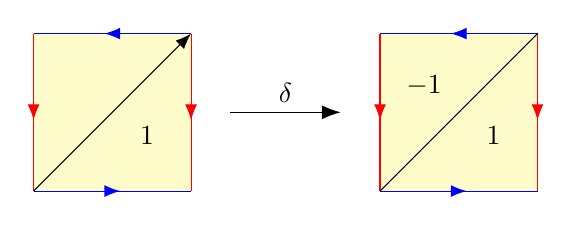
\begin{tikzpicture}[scale=2]
  \kleinsq{0}
  \draw[-{Latex[length=2mm]}] (0,0) -- (1,1);
  \node at (0.72,0.35) {$1$};
  \draw[-{Latex[length=2.4mm]}] (1.25,0.5) -- (1.95,0.5) node[midway, above] {$\delta$};
  \kleinsq{2.2}
  \draw (3.2,1) -- (2.2,0);
  \node at (2.92,0.35) {$1$};
  \node at (2.48,0.67) {$-1$};
\end{tikzpicture}
\end{document}
